\chapter{Proposed Solution: Workflow-First Deployment via Function Registry Resolution}
\label{ch:proposed_solution}

This chapter introduces the core idea of the proposed OmniFlow-QuickFaaS integration. The objective is to reduce the manual work required to deploy workflows that depend on serverless functions, while keeping the workflow definition readable and stable.

In the reference OmniFlow usage, a \texttt{Call} step is expressed as an HTTP request where the developer provides concrete invocation details such as \texttt{method}, \texttt{host} and \texttt{path}. This implies that, when the workflow calls a serverless function, the developer must already know the function endpoint and keep it synchronized with deployments. The proposed solution streamlines this experience by letting the developer declare an internal function call directly on the call step, through a dedicated \texttt{internalFunction(name, deploymentDescriptorPath)} construct, mutually exclusive with the plain \texttt{host}/\texttt{path} fields used for external calls. This enables a single workflow-first deployment that resolves (or, if needed, provisions) the required internal functions and then deploys the workflow to the chosen cloud provider.

\section{Components Architecture}
\label{sec:components-architecture}

The proposed integration keeps the original OmniFlow workflow model but extends the toolchain with a small set of additional components that cooperate at deployment time. The goal is to allow the developer to start from a single workflow definition and obtain both the deployed workflow and the deployed internal functions on a single cloud provider, without manually copying endpoints into the DSL.

Figures~\ref{fig:architecture-before} and~\ref{fig:architecture-after} contrast the developer workflow before and after the integration proposed in this dissertation.

In the prior state (Figure~\ref{fig:architecture-before}), OmniFlow and QuickFaaS are used independently. The developer first deploys each function with QuickFaaS in a separate manual step, retrieves the resulting invocation endpoint, and copies it by hand into the workflow definition before deploying the workflow. This manual synchronisation is error-prone: any redeployment that changes an endpoint forces a corresponding edit to the workflow. Moreover, QuickFaaS targeted only GCP and Azure, so along the AWS path OmniFlow had no function-deployment capability at all — the corresponding extension point was occupied by a no-op placeholder (\texttt{NoopInternalFunctionDeployer}). The two lifecycle concerns, function deployment and workflow deployment, are therefore completely disconnected.

\begin{figure}[htbp]
  \centering
  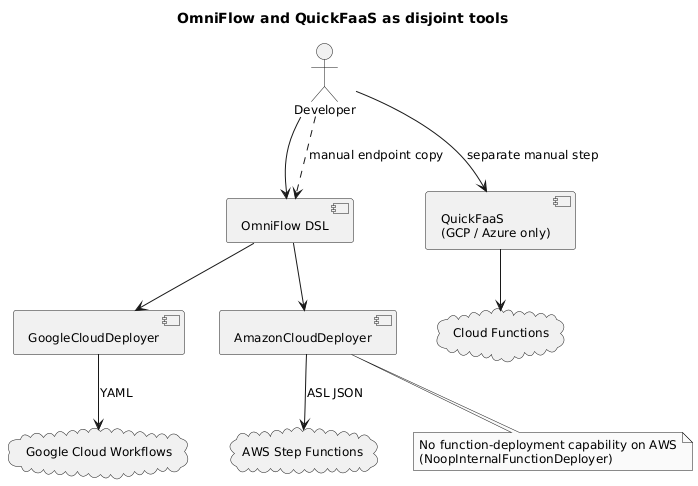
\includegraphics[width=0.85\textwidth]{images/architecture/architecture-before.png}
  \caption{OmniFlow and QuickFaaS operate as two disjoint tools.}
  \label{fig:architecture-before}
\end{figure}

In the state introduced by this work (Figure~\ref{fig:architecture-after}), a single workflow definition drives both concerns. Each provider deployer delegates internal-call resolution to a provider-specific resolver — \texttt{WorkflowInternalFunctionResolver} for GCP and \texttt{AwsInternalFunctionResolver} for AWS — and both are backed by a shared \texttt{function-registry.json} that maps logical identifiers to concrete invocation metadata. QuickFaaS is extended with an \texttt{AwsProvider}, so a function can be deployed on demand to AWS Lambda through the same subprocess mechanism already used for GCP. Once resolved, the rendered Step Functions state machine invokes the Lambda natively by ARN. The two halves of the contribution are visible in a single view: the AWS provider inside QuickFaaS (Part~A) and the resolver–registry layer that unifies function and workflow deployment (Part~B).

\begin{figure}[htbp]
  \centering
  
\includegraphics[width=\textwidth]{images/architecture/architecture-after.png}
  \caption{Unified deployment driven from a single workflow definition; components marked as new/extended are the contribution of this work (Parts~A and~B).}
  \label{fig:architecture-after}
\end{figure}

The end-to-end flow proceeds as follows: (1) the developer defines the workflow and one QuickFaaS descriptor per internal function; (2) OmniFlow parses the workflow and, for each internal call, (3) resolves the endpoint from the registry, discovers it directly on the provider, or deploys it through QuickFaaS; (4) the returned metadata is written to the registry; and (5) the resolved workflow is rendered and deployed to the provider's workflow service. External calls bypass the registry entirely.

\section{Design Rationale: Embedding Function Deployment in OmniFlow}
\label{sec:design-rationale}

A central design decision of this integration is that OmniFlow \emph{drives} QuickFaaS as part of a
single workflow deployment, rather than the two tools being deployed as independent, long-running
services that communicate over a network API. This section justifies that choice and states its
trade-offs explicitly.

\paragraph{Why OmniFlow orchestrates QuickFaaS.}
The objective of this work is a \emph{workflow-first} deployment: the developer starts from one
workflow definition and OmniFlow makes the referenced internal functions available before deploying
the workflow. Only OmniFlow has the information needed to drive this flow --- it owns the
deployment entry point and the workflow tree, and therefore knows which internal functions the
workflow references and in what order they must be resolved. QuickFaaS, by contrast, operates at the
granularity of a single function described by a deployment descriptor and has no notion of a
workflow. The orchestration must therefore live on the OmniFlow side, with QuickFaaS acting as the
function-deployment mechanism it invokes on demand. Crucially, this is a \emph{deployment-time},
client-side, one-shot action performed on the developer's machine, not a recurring runtime
interaction between two systems.

To keep the two tools decoupled despite this dependency, function deployment is reached through the
\texttt{InternalFunctionDeployer} strategy interface, whose provider implementations
(\texttt{QuickFaasDeployer} for GCP, \texttt{AwsLambdaDeployer} for AWS) invoke QuickFaaS as an
external process. QuickFaaS is thus reused as-is, remaining a separately owned and separately built
tool (its own repository, Gradle build and Kotlin~1.6.20 toolchain), instead of having its source
merged into OmniFlow's Maven build.

\paragraph{Why not two independent communicating services.}
An alternative design would run OmniFlow and QuickFaaS as two standing services that exchange
messages over a network. This was rejected for several reasons. First, neither tool is a
long-running service: OmniFlow is a client-side library invoked during a build, and QuickFaaS is a
self-contained desktop application that consumes a local deployment descriptor and exposes no
network API. Turning either into a service would require re-architecting it and then hosting,
securing and keeping it available. Second, doing so would reintroduce precisely the
``additional runtime layer that must be operated'' which this thesis deliberately avoids
(Chapter~\ref{ch:related-works}): the contribution is aligned with provider-native execution
surfaces and adds no new infrastructure of its own. Third, deployment uses the developer's own
cloud credentials, resolved locally (e.g., application-default credentials or environment
variables); a service-to-service design would have to transport or delegate those credentials
across a trust boundary, a security liability with no corresponding benefit for a single-developer,
single-machine build. Finally, for a task that is inherently sequential, local and ephemeral, a
direct invocation has far fewer failure modes than a distributed protocol (no network partitions,
partial failures, or inter-service API to version), and the coupling is in fact looser --- OmniFlow
depends on the QuickFaaS build artifact, not on a running service.

\paragraph{Trade-off of the current mechanism.}
In the present prototype the invocation is realised as a subprocess: OmniFlow places the deployment
descriptor (and the function source) next to the QuickFaaS JAR and launches it with
\texttt{java\ -jar}, detecting success from the process exit code and a marker printed on its
output. This is pragmatic --- it reuses QuickFaaS's existing headless entry point without modifying
it --- but it is also the most brittle part of the integration, since it couples the two build
systems at run time through a JAR path and parses the child process's output. Importantly, the
cleaner alternative to the subprocess is \emph{in-process library invocation} (linking QuickFaaS as
a dependency), which preserves the OmniFlow-drives-QuickFaaS model while removing the process
boundary; this is discussed as future work (Chapter~\ref{cha:conclusions}) and is a different axis
from the two-service design rejected above.

\section{DSL Extensions}
\label{sec:dsl-extensions}

The OmniFlow background chapter described how a workflow is modelled as a tree of \texttt{Step} nodes, each with a single \texttt{context} that determines its behaviour (Call, Assign, Switch, Iteration, Parallel). Within this hierarchy, \emph{execution steps} correspond to nodes that actually perform work (such as HTTP calls or variable assignments). This section focuses on one particular execution step, the \texttt{call} step, and on how it is extended in this dissertation.

Figure~\ref{fig:call-step-model} shows how the \texttt{call} step is extended to express internal function calls. In the original design, a \texttt{CallContext} carries the literal HTTP fields \texttt{host} and \texttt{path}. This work adds an optional association to an \texttt{InternalFunction}, which holds a logical \texttt{name} (the \texttt{functionRef}) and an optional \texttt{deploymentDescriptorPath}. The two construction paths are \emph{mutually exclusive}, as captured by the XOR invariant: an external call provides \texttt{host}/\texttt{path} and no \texttt{internalFunction}; an internal call provides an \texttt{internalFunction} and \emph{must not} set \texttt{host} or \texttt{path}, since those are injected automatically at deployment time by the resolution mechanism. This invariant is enforced twice — first by the DSL builder, which rejects the illegal combination at construction time, and again defensively by the resolvers before rendering — so an ambiguous call definition can never reach the provider artifact. Keeping the internal form as an alternative on the existing step, rather than introducing a new step type, means developers continue to describe calls with the familiar HTTP vocabulary.

\begin{figure}[htbp]
  \centering
  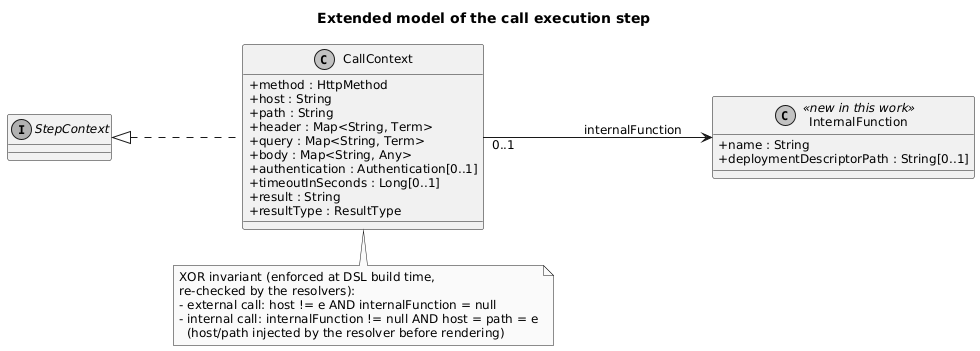
\includegraphics[width=0.8\textwidth]{images/dsl-extension/call-step-model.png}
  \caption{Extended model of the \texttt{call} execution step, with the mutually
  exclusive \texttt{internalFunction} association added in this work.}
  \label{fig:call-step-model}
\end{figure}

The proposed solution introduces \texttt{internalFunction}(name, deploymentDescriptorPath) as an alternative construction path for the call step, mutually exclusive with \texttt{host}/\texttt{path}. Setting \texttt{internalFunction} declares that this call targets a function owned by the developer; \texttt{host} and \texttt{path} are then filled in automatically by OmniFlow at deployment time and must not be provided in the DSL. The optional second parameter, \texttt{deploymentDescriptorPath}, points to a QuickFaaS deployment descriptor and is consulted only if the function cannot be resolved from the registry or discovered directly on the target provider.

With this extension, the call step can be used in two distinct ways:

\begin{itemize}
  \item For \textbf{external calls}, the call step is used exactly as in the original OmniFlow design: \texttt{method}, \texttt{host} and \texttt{path} are mandatory and contain a concrete HTTP endpoint; \texttt{internalFunction} is omitted and no function deployment is triggered by the integration.
  \item For \textbf{internal calls}, the developer omits \texttt{host}/\texttt{path} and instead sets \texttt{internalFunction(name, deploymentDescriptorPath)}. The call targets a function owned by the developer; its concrete endpoint is resolved at deployment time (and the function deployed via the descriptor if necessary) and injected into the rendered workflow.
\end{itemize}

By introducing \texttt{internalFunction} directly in the call execution step, the DSL remains close to the original OmniFlow design—developers still describe calls using the familiar step vocabulary—while gaining a clear hook that connects internal calls to the QuickFaaS-based deployment and registry mechanisms described in the following sections.

The main DSL-related concepts can be summarised as follows:

\paragraph{Internal Function.}
An internal function is a function owned by the workflow developer. The developer controls its source code and is allowed to deploy and update it. In the proposed integration, only internal functions are managed by QuickFaaS and stored in the Function Registry.

\paragraph{External Function.}
An external function is a function or API not owned by the workflow developer (for example, developed by a third party). The workflow developer is not allowed to deploy or update it. External functions are treated as unmanaged HTTP dependencies, OmniFlow may invoke them using literal \texttt{host/path} fields, but QuickFaaS must not be used to deploy or update them and they are not recorded in the registry.

\paragraph{Function Reference (\texttt{functionRef}).}
A function reference (\texttt{functionRef}) is a stable logical identifier used to name an internal function (e.g., \texttt{"fraud-check"}). This identifier is used consistently across the workflow definition, the registry metadata and the deployment descriptors. It is not an endpoint, it is a name that allows OmniFlow to bind a call to the concrete endpoint during deployment.

\paragraph{Function Registry.}
The function registry is a file that contains invocation metadata only for internal functions. Conceptually, it maps each internal \texttt{functionRef} to the concrete values required to invoke it. These values are not written manually; when an internal function is deployed or updated through QuickFaaS, the integration records or refreshes the corresponding entry in the registry. External functions are excluded from the registry. A minimal JSON-based structure for this registry is illustrated in Listing~\ref{lst:registry-structure}.

\begin{lstlisting}[caption={Example structure of the function registry (internal functions only).},label={lst:registry-structure},basicstyle=\ttfamily\small,breaklines=false]
{
  "updatedAt": "2026-02-12T18:40:00Z",
  "functions": {
    "fraud-check": {
      "serviceName": "fraud-check",
      "url": "https://fraud-check-abc123-ew.a.run.app/v1/fraud-check"
    },
    "hello-lambda-fn": {
      "serviceName": "hello-lambda-fn",
      "url": "arn:aws:lambda:eu-west-1:123456789012:function:hello-lambda-fn"
    }
  }
}
\end{lstlisting}

Listing~\ref{lst:call-step-internal} shows a call step that targets an internal function.

\begin{lstlisting}[language=Kotlin,caption={Call step declaring an internal function via \texttt{internalFunction}.},label={lst:call-step-internal}]
step {
  name("call-auto-deployed-function")
  description("Calls a function that QuickFaaS will deploy if not already running")
  context(
    call {
      method(GET)
      internalFunction(
        "quickfaas-test-fn",
        deploymentDescriptorPath = "./functions/quickfaas-test-fn/func-deployment.json"
      )
      result("result")
    }
  )
}
\end{lstlisting}

\paragraph{QuickFaaS Deployment Descriptor and Code File}
To deploy (or update) an internal function, QuickFaaS requires two artifacts: (i) a JSON deployment descriptor and (ii) the function code file. The descriptor specifies the deployment parameters and also points to the code file through the \texttt{functionFile} field, which is a filesystem path to the function implementation. Listing~\ref{lst:quickfaas_json_config} in section \ref{sec:background_quickfaas} is an example of the deployment descriptor.

\section{Developer Procedure for Deploying a Workflow}
\label{sec:developer-workflow}

To deploy a workflow that introduces one new internal function and calls one external function, the developer prepares a QuickFaaS deployment descriptor file (JSON) for the internal function and the corresponding code file referenced by \texttt{functionFile}. The descriptor defines the provider, project, location and function settings (name, runtime, trigger, bucket) and points to the implementation file path, which is the second required input for deployment. No QuickFaaS descriptor is created for the external function because the developer is not its owner and the integrated tool must not deploy or update it.

Because internal calls are declared with \texttt{internalFunction("fraud-check", ...)} rather than a concrete endpoint, the developer only needs to choose a stable \texttt{functionRef} and use it consistently in the workflow and in the QuickFaaS descriptor. Read access to the Function Registry is useful to discover which internal functions already exist and which \texttt{functionRef} identifiers are already in use, but it is not required for a brand-new function: after the first integrated deployment, OmniFlow records the binding so the same \texttt{functionRef} can be reused reliably in future workflows.

The workflow is written as shown in Listing~\ref{lst:wf-internal-part} and Listing~\ref{lst:wf-external-part}. Listing~\ref{lst:wf-internal-part} shows the first step, which calls an internal function: instead of a concrete endpoint it uses \texttt{internalFunction("fraud-check", "./deploy/fraud-check.json")}, whose second argument points to the QuickFaaS descriptor. Listing~\ref{lst:wf-external-part} completes the workflow with a second step that calls an external API using literal \texttt{host}/\texttt{path} values and no \texttt{internalFunction}. When the integrated deployment runs, OmniFlow resolves (and, if needed, deploys) only the internal call, updates the registry, injects the resolved endpoint, and finally deploys the workflow. The external call is left unchanged and is not stored in the registry.

\begin{lstlisting}[language=Kotlin,caption={FraudPipeline workflow (part 1/2): internal function call.},label={lst:wf-internal-part},basicstyle=\ttfamily\small,breaklines=false]
val wf = workflow {
  name("FraudPipeline")
  input("args")
  steps(
    step {
      name("fraud-check")
      context(call {
        method(GET)
        internalFunction("fraud-check", "./deploy/fraud-check.json")
        result("fraudResult")
      })
    },
    ...
\end{lstlisting}

\begin{lstlisting}[language=Kotlin,caption={FraudPipeline workflow (part 2/2): external function call.},label={lst:wf-external-part},basicstyle=\ttfamily\small,breaklines=false]
...
// FraudPipeline workflow (continuation)
    step {
      name("external-risk-api")
      context(call {
        method(POST)
        host("api.partner.example")
        path("/v1/risk-score")
        result("riskResult")
      })
    }
  )
  result("riskResult")
}
\end{lstlisting}












